% !TEX TS-program = xelatex
% !TEX encoding = UTF-8 Unicode

% In Class Activity for ME3001- Tristan Hill 
% Spring 2017 - Fall 2017 - Fall 2020 - Fall 2021
% Mechanical Engineering Analysis with MATLAB  and Solidworks
% Module 1 - Deisgn with Solidworks
% Activity 3 -(In-Class)- Introduction to Solidworks 

\documentclass[12pt]{article}
\usepackage{/home/thill/Documents/lectures/analysis_lectures/analysis_activities}

% Title and Misc
\newcommand{\COURNAME}{ME 3001-002}
\newcommand{\CURRTERM}{Fall 2021} %Current Term
\newcommand{\MNUM}{1} %Module Number
\newcommand{\ANUM}{6} %Activity Number
\newcommand{\moduletitle}{Systems of Linear Equations}
\newcommand{\activitytitle}{Scaffolding Analysis} %Module Name
\pagestyle{myheadings}
%\markright{{\large ME4140 - ROS Workshop - \CURRTERM}}

\textwidth=7.0in
\topmargin=-0.6in
\leftmargin=0.5in
\textheight=9.25in
\hoffset=-0.5in
\footskip=0.2in

\begin{document}

\thispagestyle{plain}

\begin{center}
   {\bf \Large In-Class Activity\hspc\ANUM\hspc - \activitytitle}\vspace{3mm}\\
   {\bf \large \COURNAME - Mechanical Engineering Analysis - \CURRTERM} \vspace{5mm}\\
\end{center}

\begin{description}


\item[\textbf{\underline{Learning Objectives:}}] \hfill \vspace{0mm}

\begin{itemize}
	\item Demonstrate deriving a system of ,linear equations to represent a static analysis.
	\item Demonstrate converting a system of linear equations into matrix form.
	\item Practice using linear algebra techniques in MATLAB to solve an applied engineering problem.
\end{itemize}


\item[\textbf{\underline{Overview:}}] \hfill \vspace{3mm}\\

As an engineer you are asked to analyze the simple scaffolding structure shown. The rigid structure above rests on the ground in static equilibrium. 

\item[\textbf{\underline{Overview:}}] \hfill \vspace{3mm}\\
	
	
	
	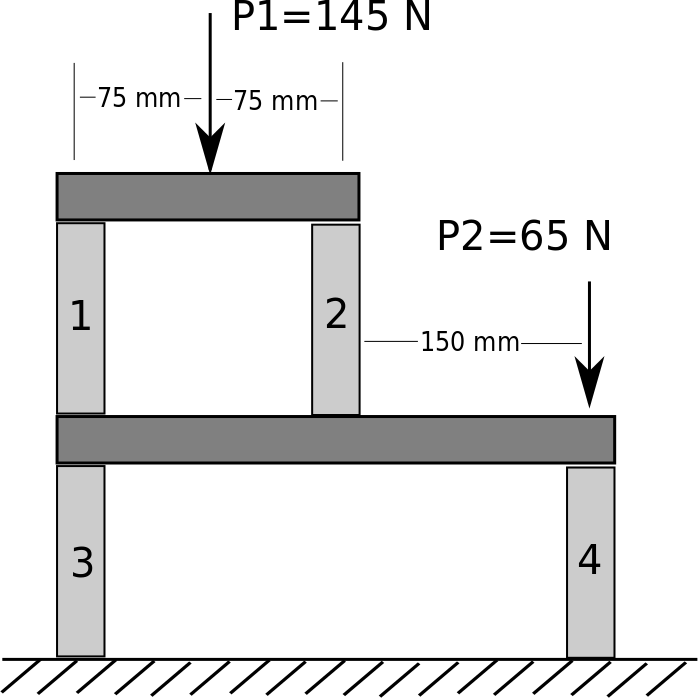
\includegraphics[scale=.25]{activity6_fig1.png}\\
	
	\item[\textbf{\underline{Required Materials:}}] \hfill \vspace{0mm}
	
	\begin{itemize}
		\item {\bf Your Computer}: This activity requires a computer with MATLAB installed.
	\end{itemize}
	
	\item[\textbf{\underline{Peer Collaboration:}}] \hfill \vspace{0mm}
	
	{\bf This is an individual assignment}, but you are encouraged to discuss the problem with your peers. You must write your own program and submit as an individual, but you can share ideas about the algorithm with your peers and the instructor.

\newpage	
\item[\textbf{\underline{Analysis Requirements:}}] \hfill \vspace{0mm}

	
	\begin{itemize}
		
	\item Write 2 static equilibrium equations for bar 1 and bar 2 each for a total of 4 equations. Show the equations with unknowns in order and the knowns on the right hand side.\vspace{10mm} \\
	
	%   \scalebox{1}{$KVL_1=-v_a+R_1\times i_1-(i_1-i_2)\times R_2 =0$} \vspace{3mm} \vspace{30mm}
	
	\item Cast the system of equations into matrix form. Be sure to label the {\it Coefficient Matrix}, {\it The Vector of Knowns}, and {\it The Vector of Unknowns}. Also, please write the unknown vector with the loads in order (1,2,3,4).\vspace{10mm}
	
	
	\item Solve for the unknowns using the matrix inverse. 
	
	\end{itemize}


\item[\textbf{\underline{Activity:}}] \hfill \vspace{0mm}

\begin{enumerate}
	

	\item Write a MATLAB program to solve the static analysis problem described on the previous page. {\it Remember to put a proper header at the top of your main program, and clear the workspace in the script directly below the header. } The main file of your program should be called {\bf \BL<USERNAME>\BK\_activity\ANUM.m}
	
	
	\item Write a brief description of how your program works to solve the problem. This can be a few sentences or a bulleted list. Also include the analysis results in  {\bf \BL<USERNAME>\BK\_activity\ANUM.pdf }.
	
	
\end{enumerate}

\item[\textbf{\underline{Submit:}}] \hfill \vspace{0mm}

		Submit the most complete version of {\bf \BL<USERNAME>\BK\_activity\ANUM.pdf} \\and {\bf \BL<USERNAME>\BK\_activity6.m } to the Activity \ANUM \hspace{1mm} folder before the posted due date.

\end{description}
\end{document}
